% main.tex — 日本語本文(LuaLaTeX + luatexja 推奨)
% ビルド例: lualatex main.tex ; lualatex main.tex
\documentclass[11pt,a4paper]{ltjsarticle} % LuaLaTeX + luatexjaクラス

% 版面
\usepackage{geometry}
\geometry{margin=22mm}

% 数値・単位
\usepackage{siunitx}
\sisetup{detect-all=true}

% 図表・色
\usepackage{graphicx}
\usepackage{booktabs}
\usepackage{xcolor}
\usepackage{caption}
\usepackage{subcaption}

% ハイパーリンク
\usepackage{hyperref}
\hypersetup{
  colorlinks=true,
  linkcolor=blue,
  urlcolor=blue,
  citecolor=blue,
  pdfauthor={Shinichi Samizo},
  pdftitle={PZT薄膜アクチュエータにおける振動板クラックと端部焼損の原因解析・対策提案}
}

% 図の描画(TikZ)
\usepackage{tikz}
\usetikzlibrary{arrows.meta,calc}

% 外部TikZの取り込み(無くてもビルドできるよう保険)
\usepackage{standalone}
\usepackage{upquote}

%======== 図プレースホルダ(外部figsが無い場合でもビルド可能にする) ========%
% \IfFileExists は LaTeX 標準
\newcommand{\figVoidDonut}{%
  \IfFileExists{figs/fig1_void_donut.tikz}{%
    \input{figs/fig1_void_donut.tikz}%
  }{%
    % 代替の簡易ドーナツ図
    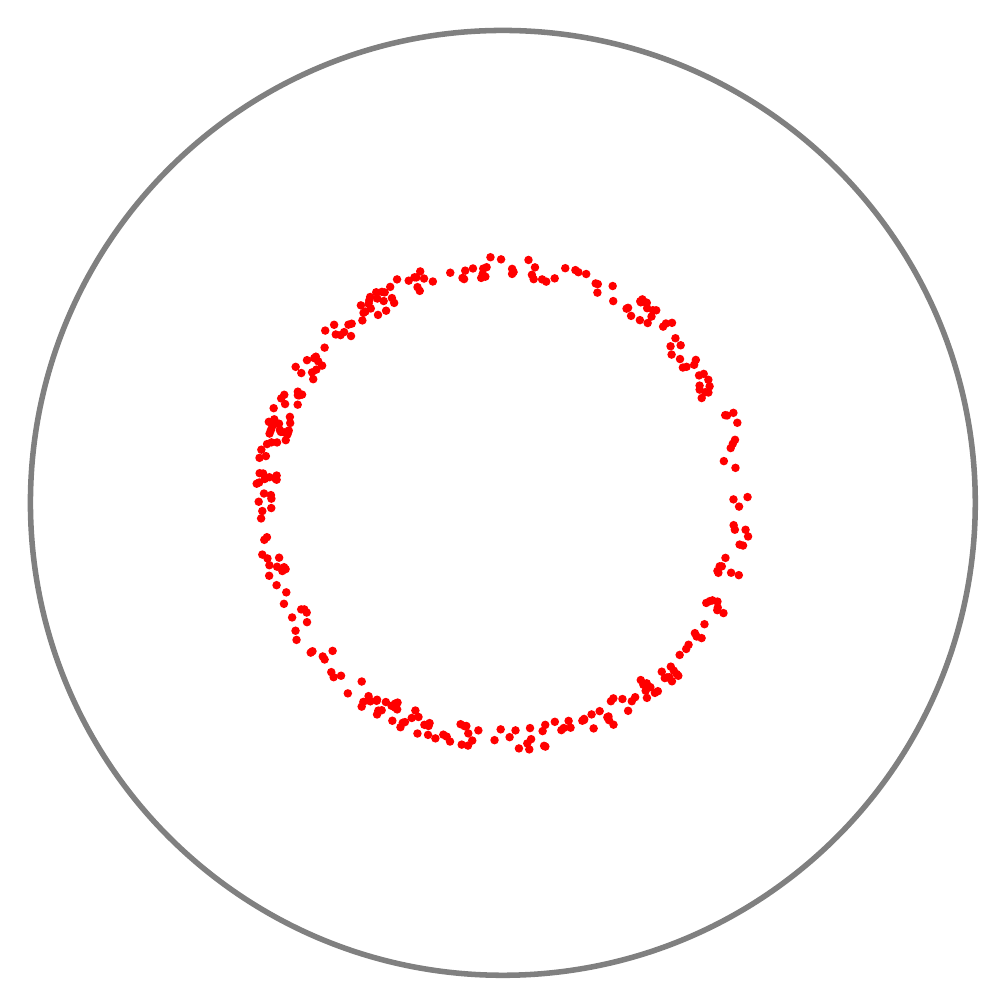
\begin{tikzpicture}[scale=0.06]
      \draw[line width=2pt, gray] (0,0) circle (100);
      \foreach \i in {1,...,320}{
        \pgfmathsetmacro{\ang}{rnd*360}
        \pgfmathsetmacro{\rad}{50 + 5*(rnd-0.5)}
        \fill[red] (\ang:\rad) circle (0.9);
      }
    \end{tikzpicture}%
  }%
}

\newcommand{\figPZTLayersVoid}{%
  \IfFileExists{figs/fig2_pzt_layers_void.tikz}{%
    \input{figs/fig2_pzt_layers_void.tikz}%
  }{%
    % 代替の6層+1層ボイド断面
    \begin{tikzpicture}[x=1cm,y=1cm]
      \def\W{6.0}\def\H{0.45}\def\G{0.10}
      \foreach \i in {0,...,5}{
        \pgfmathsetmacro{\y}{\i*(\H+\G)}
        \draw[fill=gray!20] (0,\y) rectangle (\W,\y+\H);
      }
      % 4層目に矩形ボイド
      \pgfmathsetmacro{\yv}{3*(\H+\G)}
      \draw[very thick,red] (2.2,\yv+0.10) rectangle (3.0,\yv+\H-0.10);
      % 上下に細線(電極/基板イメージ)
      \draw[line width=1pt] (0,-0.30) -- (\W,-0.30);
      \draw[line width=1pt] (0,6*(\H+\G)+0.10) -- (\W,6*(\H+\G)+0.10);
    \end{tikzpicture}%
  }%
}

\newcommand{\figEdgeBurnout}{%
  \IfFileExists{figs/fig3_edge_burnout_color.tikz}{%
    \input{figs/fig3_edge_burnout_color.tikz}%
  }{%
    % 代替の端部焼損模式図(カラー)
    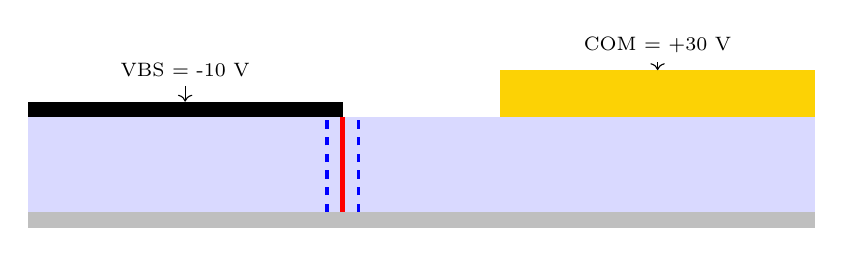
\begin{tikzpicture}[x=1cm,y=1cm]
      \def\W{10}\def\pztH{1.2}\def\beH{0.2}\def\teH{0.20}
      % Bottom Electrode
      \fill[gray!50] (0,0) rectangle (\W,\beH);
      % PZT
      \fill[blue!15] (0,\beH) rectangle (\W,\beH+\pztH);
      % Top Electrode (VBS)
      \fill[black] (0,\beH+\pztH) rectangle (4,\beH+\pztH+\teH);
      % Au Pad (COM)
      \fill[yellow!70!orange] (6,\beH+\pztH) rectangle (\W,\beH+\pztH+0.6);
      % Exposed sidewall
      \draw[line width=1.8pt,red] (4,\beH) -- (4,\beH+\pztH);
      % Proposed AlOx
      \draw[line width=1.2pt,blue,dashed] (3.8,\beH) -- (3.8,\beH+\pztH);
      \draw[line width=1.2pt,blue,dashed] (4.2,\beH) -- (4.2,\beH+\pztH);
      % Voltage labels(英数字のみでフォント依存回避)
      \draw[->] (2, \beH+\pztH+\teH+0.2) -- (2,\beH+\pztH+\teH);
      \node[anchor=south] at (2, \beH+\pztH+\teH+0.2) {\scriptsize VBS = -10 V};
      \draw[->] (8, \beH+\pztH+0.7) -- (8,\beH+\pztH+0.6);
      \node[anchor=south] at (8, \beH+\pztH+0.7) {\scriptsize COM = +30 V};
    \end{tikzpicture}%
  }%
}

%======== タイトル情報 ========%
\title{PZT薄膜アクチュエータにおける振動板クラックと端部焼損の原因解析・対策提案}
\author{三溝 真一(Shinichi Samizo)\\
Independent Semiconductor Researcher\\
Former Engineer at Seiko Epson Corporation\\
\href{mailto:shin3t72@gmail.com}{shin3t72@gmail.com}\quad
GitHub: \url{https://github.com/Samizo-AITL}}
\date{} % 必要なら提出日

\begin{document}
\maketitle

\begin{abstract}
本論文は、Epson $\mu$TFP(薄膜PZT $d_{33}$)アクチュエータユニットにおいて顕在化した
(1) 振動板クラック不良および (2) セグメント端部の焼損不良
の二課題について、現象・原因・対策を横断的に整理したものである。
ユニットスクリーニング時に多発したクラックは、RTA後の表面疎水化に起因するスピン塗布時の気泡巻き込み(\emph{膜内ボイド化})が原因であり、
酢酸プレウェット(親水化)を恒久対策として導入し、不良率を5--10\%からほぼ0\%に低減した。
一方、端部焼損は、COM(下電極側)とVBS(上電極側)が最接近する構造における\emph{PZT側壁露出}と40\,V差(+30\,V/--10\,V)に伴う電界集中に起因すると推定し、
対策案としてALDによるAlO$_x$保護膜の付与を提示する。
\end{abstract}

\section{序論}
インクジェットプリントヘッドは、印字品質・速度・信頼性向上の要請に応え、アクチュエータ構造の世代交代を重ねてきた。
第1世代のMachヘッドはバルク積層PZT($d_{31}$、180\,dpi、ベンダー: TDK/村田)を採用していたが、高精細化には素子寸法が制約となった。
第2世代のTFP/$\mu$TFPヘッドでは、エプソン(広丘事業所)にて薄膜PZT($d_{33}$)を内製化し、300\,dpiに対応する高密度・高速応答を実現した。
一方で、薄膜化と高電界化により、膜欠陥(クラック・ボイド)および端部絶縁破壊が顕在化した。
本論文では、これらの課題をプロセス・デバイス・試験条件の観点から統合的に解析し、対策を示す。

\section{デバイス・プロセス構成}
\subsection{層構成}
アクチュエータチップの代表構成を表\ref{tab:stack}に示す。
\begin{table}[h]
  \centering
  \caption{薄膜PZTアクチュエータの代表的層構成}
  \label{tab:stack}
  \begin{tabular}{@{}lll@{}}
    \toprule
    層 & 材料 & 代表厚み \\\midrule
    Si基板((111)) & Si & --- \\
    絶縁層 & ZrO$_2$ & 400\,nm \\
    接着層 & Ti & 10\,nm \\
    下電極 & Pt(111) & 80\,nm \\
    seed層 & Ir & 10\,nm \\
    \textbf{PZT層} & Pb(Zr,Ti)O$_3$ & \textbf{200\,nm $\times$ 6 = 1.2\,\si{\micro\meter}} \\
    中間層(第1層後) & Ti & 4\,nm \\
    上電極 & Ir/Ti & 10/10\,nm \\\bottomrule
  \end{tabular}
\end{table}

\subsection{成膜と熱処理}
PZTはゾルゲル法により、\emph{スピン塗布 $\rightarrow$ プリベーク(150--200$^\circ$C)$\rightarrow$ RTA結晶化(737$^\circ$C)}を1層毎に6回繰返し、
総厚\SI{1.2}{\micro\meter}を形成する。第1層焼成後にTi \SI{4}{\nano\meter}を挿入し、組成傾斜・界面応力を緩和する。

\subsection{評価系とスクリーニング}
結晶配向はXRD($\theta$–2$\theta$)でPZT(100)を確認、膜厚/組成はXRFでインライン計測、P-E特性は$\pm$40\,V/66\,Hzで評価。
ユニットスクリーニング(ポーリング)は、\emph{DC 60\,s + AC 90\,s}(台形波)で実施し、電位条件は\emph{COM=+30\,V、VBS=--10\,V}(差分40\,V)とした。

\section{結果}
\subsection{クラック:同心リング分布と層内ボイド}
長期放置後に塗布・焼成したウェハでは、反射条件を調整したパーティクル検査において、半径中間域に\emph{ドーナツ状の欠陥分布}が観測された(図\ref{fig:donut})。
断面観察では、PZT 6層のうち\emph{特定の1層にボイド}が局在し、その位置がクラック進展起点と一致する(図\ref{fig:layer-void})。

\begin{figure}[h]
  \centering
  \figVoidDonut
  \caption{ウエハ上のドーナツ状ボイド分布(反射条件最適化による検出例)}
  \label{fig:donut}
\end{figure}

\begin{figure}[h]
  \centering
  \figPZTLayersVoid
  \caption{PZT 6層のうち1層にボイドを含む断面模式図}
  \label{fig:layer-void}
\end{figure}

\subsection{端部焼損:電界集中部位}
ユニットスクリーニング時、COM(Au配線)とVBS(上電極)が最接近する\emph{PZT側壁露出部}で焼損が発生した。
差分40\,Vの台形波立上りで瞬間電流が重畳し、局所的絶縁破壊が誘発されたと推定される(図\ref{fig:edge})。

\begin{figure}[h]
  \centering
  \figEdgeBurnout
  \caption{端部焼損の模式図(電界集中部とAlO$_x$対策案)}
  \label{fig:edge}
\end{figure}

\section{考察}
\subsection{クラック原因の連鎖}
問題のRTA装置天井側には外気排気口があり、焼成後に微量不純物がPZT表面へ付着、接触角測定で疎水化が確認された。
疎水表面では、スピン回転直前(半径中間域)に気泡取り込みが最大化し、膜内ボイドとして残存、同心リング状の欠陥分布を生じる。
\emph{酢酸プレウェット}で親水化すると、気泡巻き込みは解消し、PZT配向率・P-Eヒステリシス・吐出特性に有意差は認められなかった(No.\,1~No.\,400のセグメント間傾きも無し)。

\subsection{焼損の推定機構と対策案}
端部構造ではPZT側壁が不可避的に露出し、空気絶縁の耐圧がボトルネックとなる。
最大40\,V差の台形波立上りで電界集中が強まり、局所破壊~焼損へ至る。
\textbf{対策案}: ALDによる\emph{AlO$_x$側壁被覆}で耐圧強化、補助的に電圧条件の最適化(+25\,V/--5\,V 等)、長期的にはレイアウト変更で端部距離を稼ぐ。

\section{結論}
(1) クラックは、\emph{RTA後の疎水化 $\rightarrow$ 気泡巻き込み $\rightarrow$ 膜内ボイド}の連鎖が原因であり、酢酸プレウェット導入により不良率を5--10\%からほぼ0\%に低減し量産反映した。
(2) 端部焼損は、\emph{PZT側壁露出+電界集中}が主因と推定され、\emph{ALD-AlO$_x$被覆}を対策案として提示した。
本知見は、薄膜PZT $d_{33}$アクチュエータの高密度・高電圧駆動時における量産信頼性設計の指針となる。

\section*{著者略歴}
\textbf{三溝 真一(Shinichi Samizo)} 長野県・信州大学大学院 電子情報工学専攻 修士。
セイコーエプソンにて半導体メモリ/ミックスドシグナル開発、薄膜PZT MEMSアクチュエータおよびPrecisionCoreプリントヘッド技術に従事。
現在は独立系半導体リサーチャとして、プロセス/デバイス教育、メモリアーキテクチャ、AI統合制御に注力。
\textbf{Contact:} \href{mailto:shin3t72@gmail.com}{shin3t72@gmail.com}。

\end{document}
